\LevelOneTitle{可压缩流动基础}

\LevelTwoTitle{微弱扰动波}

\LevelThreeTitle{*什么是微弱扰动波}

\begin{definition}[微弱扰动波]\label{def11.1}
	由扰动源发出的,通过介质后状态发生微弱变化的波,其传播过程可视作一等熵过程。
\end{definition}

\LevelThreeTitle{什么是音速}

\begin{definition}[音速]
	微弱扰动波在可压缩介质中传播的速度(相对于流体介质),用$a$表示。
\end{definition}

\begin{equation}
	a = \sqrt{\dv{p}{\rho}} = \sqrt{\dfrac{E_v}{\rho}} = \sqrt{\gamma R_g T}
\end{equation}

\LevelThreeTitle{什么是马赫数}

\begin{definition}
	流速与当地音速之比,物理意义是惯性力和弹性力之比,即
	\begin{equation}
		Ma = \dfrac{V}{a}
	\end{equation}
\end{definition}

\LevelThreeTitle{微弱扰动波的传播区域}

\begin{figure}[H]
	\centering
	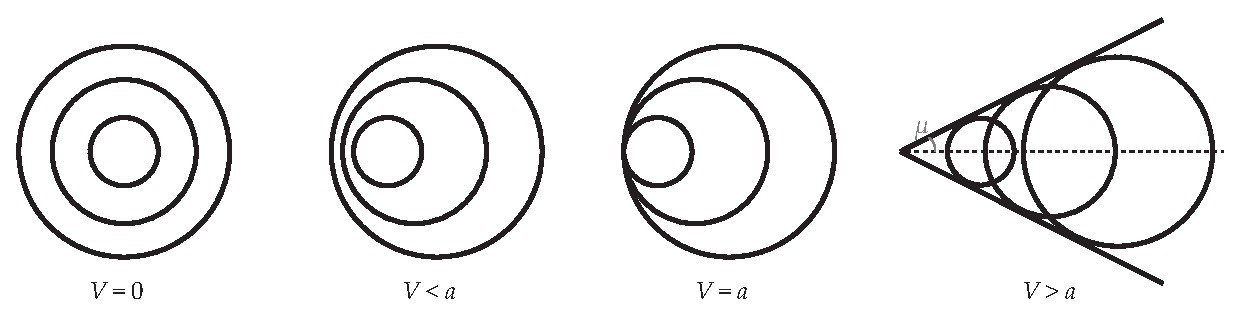
\includegraphics[scale=0.7]{figures/微弱扰动波.eps}
	\caption{微弱扰动波传播的区域}
\end{figure}

当$V > a$时,流体超音速,形成马赫角$\mu$,数学表达为

\begin{equation*}
	\mu = \arcsin(\dfrac{a}{V}) = \arcsin(\dfrac{1}{Ma})
\end{equation*}

\LevelTwoTitle{定常一元等熵流动控制方程组}

\begin{align*}
	&\rho V A = \text{const}\\
	&h + \dfrac{V^2}{2} = \text{const}\\
	&p = \rho R_g T\\
	&\dfrac{p}{\rho^{\gamma}} = \text{const}
\end{align*}

\LevelTwoTitle{三种参考状态}

\begin{enumerate}
	\item 等熵滞止状态\\
	速度滞止为零时的状态,$h_0 = h + \dfrac{V^2}{2} \Rightarrow T_0 = T + \dfrac{V^2}{2 c_p}$。
	\item 临界状态\\
	流速达到音速的状态($Ma = 1$),$T^{*} = 0.833 T_0, p^{*} = 0.528 p_0$。
	\item 极限状态\\
	温度为0 K,流速达到最大,$V_{\text{max}} = \sqrt{2h_0}$
\end{enumerate}

\LevelTwoTitle{速度系数和喷管}

\LevelThreeTitle{速度系数}

速度系数$\lambda = \dfrac{V}{a^{*}}$,物理意义是直接反映当地速度大小。

\LevelThreeTitle{喷管}

喷管的流动工况和截面变化之间的关系

\begin{equation}
	(Ma^2 - 1) \dfrac{\dd{V}}{V} = \dfrac{\dd{A}}{A}
\end{equation}

例如,当流动超音速($Ma^2 - 1 > 0$),想要让出口流速减小($\dfrac{\dd{V}}{V} < 0$),则应选择渐缩喷管($\dfrac{\dd{A}}{A} < 0$)。

喷管内流动参数变化,若$V\uparrow$,则$T, \rho, p\downarrow$;流速增大则相反,其中$p$的变化最剧烈。

\begin{enumerate}
	\item 渐缩喷管
	\begin{enumerate}
		\item $p_b \geq p^{*} \Rightarrow p_e = p_b$;
		\item $p_b < p^{*} \Rightarrow p_e = p^{*}$。
	\end{enumerate}
    \item 缩放喷管,$p_b < p^{*} \Rightarrow p_e = p_b$
\end{enumerate}

\LevelThreeTitle{个人比较喜欢的一个公式}

\begin{equation}
	\dfrac{p_e}{p_0} = \qty(1 + \dfrac{\gamma - 1}{2} Ma_e^2)^{-\frac{\gamma}{\gamma - 1}}
\end{equation}

\LevelTwoTitle{激波}

\LevelTwoTitle{*什么是激波}

\begin{definition}[激波]
	集中的有一定强度的压缩波称为激波,是由于传播速度超音速发生突跃压缩现象产生的,强间断且具有一定厚度,激波内速度梯度和温度梯度很大。
\end{definition}

\LevelThreeTitle{激波的分类}

\begin{enumerate}
	\item 正激波,波面与气流方向垂直;
	\item 斜激波,波面与气流方向不垂直;
	\item 曲面激波,波形弯曲,由正激波和斜激波构成。
\end{enumerate}

\LevelTwoTitle{正激波前后参数变化}

\begin{equation*}
	V_1 V_2 = {a^{*}}^2 \Rightarrow \lambda_1 \lambda_2 = 1
\end{equation*}

\begin{enumerate}
	\item 静参数变化\\
	$V, Ma \downarrow, T, p, \rho, a \uparrow$;
	\item 滞止参数变化\\
	$T_0$不变,$p, \rho \downarrow$;
	\item 临界参数变化\\
	$T^{*}$不变,$p, \rho \downarrow$。
\end{enumerate}

\LevelTwoTitle{例题练习}

\begin{example}
	一真空箱通过收缩形喷管从大气吸气,喷管最小截面直径为38 mm,若大气压强为101.3 kPa,温度为15 $^{\circ}$C,要使喷管出口为音速流动,真空箱压强应保持为多少?此时质量流量多少?若真空箱内压强为$0.34 \times 10^5$ Pa,质量流量为多少?
	\vskip 0.3cm
	由于是从大气吸气,因此入口参数为滞止参数,则
	\begin{equation*}
		p^{*} = 0.528 p_0 = 0.528 \times 101.3 \mathrm{~kPa} = 53.486 \mathrm{~kPa}
	\end{equation*}

	由题意,$V_e = a^{*}$,则$p_e = p^{*} = p_b$。	
	\vskip -0.3cm
    \begin{align*}
    	&T^{*} = 0.833 T_0 = 0.833 \times (15 + 273.15) \mathrm{~K} = 240 \mathrm{~K}\\
    	&\rho^{*} = \dfrac{p^{*}}{R_g T^{*}} = \dfrac{53.486 \times 10^3}{287 \times 240} \mathrm{~kg/m}^3 = 0.7765 \mathrm{~kg/m}^3\\
		&a^{*} = \sqrt{\gamma R_g T} = \sqrt{1.4 \times 287 \times 240} \mathrm{~m/s} = 310.5 \mathrm{~m/s}\\
		&\dot{m} = \rho^{*} A_e a^{*} = \dfrac{\pi \rho^{*} d_e^2 a^{*}}{4} = \dfrac{\pi \times 0.7765 \times 0.038^2 \times 310.5}{4} \mathrm{~kg/s} = 0.2734 \mathrm{~kg/s}
	\end{align*}

	若$p_b = 34$ kPa $< p^{*}$,则$p_e = p^{*}$,于是$\dot{m} = 0.2734 \mathrm{~kg/s}$不变。
\end{example}

\begin{example}
	大容器内温度为20 $^{\circ}$C的空气以1.2 kg/s的流量通过缩放喷管,喷管出口截面压强和马赫数分别是14 kPa和2.8,试确定喷管喉部和出口面积、喉部压强、出口气流速度。
	\vskip 0.3cm
	
	\begin{equation*}
		\dfrac{p_e}{p_0} = \qty(1 + \dfrac{\gamma - 1}{2} Ma_e^2)^{-\frac{\gamma}{\gamma - 1}} \Rightarrow p_0 = 379.94 \mathrm{~kPa}\\
	\end{equation*}
	
	由于$Ma_e > 1$,则喉部必达临界状态,喉部压强$p^{*} = 0.528 p_0 = 0.528 \times 379.94 \mathrm{~kPa}$。
	
	\begin{align*}
		&T_e = T_0\qty(\dfrac{p_e}{p_0})^{\frac{\gamma - 1}{\gamma}} = 290.15 \times \qty(\dfrac{14}{379.94})^{\frac{0.4}{1.4}} \mathrm{~K} = 112.99 \mathrm{~K}\\
		&a_e = \sqrt{\gamma R_g T_e} = \sqrt{1.4 \times 287 \times 112.99} \mathrm{~m/s} = 213.07 \mathrm{~m/s}\\
		&V_e = Ma_e \cdot a_e = 2.8 \times 213.07 \mathrm{~m/s} = 596.6 \mathrm{~m/s}\\
		&\rho_e = \dfrac{p_e}{R_g T} = \dfrac{14000}{287 \times 112.99} \mathrm{~kg/m}^3 = 0.4317 \mathrm{~kg/m}^3\\
		&A_e = \dfrac{\dot{m}}{\rho_e V_e} = \dfrac{1.2}{0.4317 \times 596.6} \mathrm{~m}^2 = 4.659 \times 10^{-3} \mathrm{~m}^2\\
		&T^{*} = T_0\qty(\dfrac{p^{*}}{p_0})^{\frac{\gamma - 1}{\gamma}} = 290.15 \times \qty(\dfrac{200.61}{379.94})^{\frac{0.4}{1.4}} \mathrm{~K} = 241.76 \mathrm{~K}\\
    	&\rho^{*} = \dfrac{p^{*}}{R_g T} = \dfrac{200610}{287 \times 241.76} \mathrm{~kg/m}^3 = 2.891 \mathrm{~kg/m}^3\\
    	&a^{*} = \sqrt{\gamma R_g T} = \sqrt{1.4 \times 287 \times 241.76} \mathrm{~m/s} = 311.67 \mathrm{~m/s}\\
    	&A_{\text{min}} = \dfrac{\dot{m}}{\rho^{*} a^{*}} = \dfrac{1.2}{2.891 \times 311.67} \mathrm{~m}^2 = 1.332 \times 10^{-3} \mathrm{~m}^2
    \end{align*}
\end{example}